%%% LaTeX Template: Article/Thesis/etc. with colored headings and special fonts
%%%
%%% Source: http://www.howtotex.com/
%%% Feel free to distribute this template, but please keep to referal to http://www.howtotex.com/ here.
%%% February 2011
%%%
%%% Modified May 2018 by CDM
%%% Modified/simplified by CTC 2018 - 2023

%%%  Preamble
\documentclass[11pt,letterpaper]{article}
\usepackage[margin=1.0in]{geometry}
\usepackage[T1]{fontenc}
\usepackage[bitstream-charter]{mathdesign}
\usepackage[latin1]{inputenc}					
\usepackage{amsmath}						
\usepackage{xcolor}
\usepackage{cite}
\usepackage{hyphenat}
\usepackage{graphicx}
\usepackage{float}
\usepackage{subfigure}
\usepackage{sectsty}
\usepackage[compact]{titlesec} 
\usepackage[tablegrid]{vhistory}
\allsectionsfont{\color{accentcolor}\scshape\selectfont}

%%% Definitions
%%%%%%%%%%%%%%%%%%%%%%%%%%%%%%%%%%%%%%%%%%%%%%%%%%
% Change me to fit your team/semester information

\definecolor{accentcolor}{rgb}{0.0,0.0,0.5} 
\newcommand{\teamname}{Team TLC}               %just to fill the line
\newcommand{\productname}{Roam\_Bot} 
\newcommand{\coursename}{CSE 4316: Senior Design I}
\newcommand{\semester}{Fall 2024}
\newcommand{\docname}{System Requirements Specification}
\newcommand{\department}{Department of Computer Science \& Engineering}
\newcommand{\university}{The University of Texas at Arlington}
\newcommand{\authors}{Abubakar Kassim \\ Andrew Howard \\ Christopher Davis \\ Madison Gage \\ Raya Sultan \\}

%%% Headers and footers
\usepackage{fancyhdr}
	\pagestyle{fancy}						% Enabling the custom headers/footers
\usepackage{lastpage}	
	% Header (empty)
	\lhead{}
	\chead{}
	\rhead{}
	% Footer
	\lfoot{\footnotesize \teamname \ - \semester}
	\cfoot{}
	\rfoot{\footnotesize page \thepage\ of \pageref{LastPage}}	% "Page 1 of 2"
	\renewcommand{\headrulewidth}{0.0pt}
	\renewcommand{\footrulewidth}{0.4pt}

%%% Change the abstract environment
\usepackage[runin]{abstract}			% runin option for a run-in title
%\setlength\absleftindent{30pt}			% left margin
%\setlength\absrightindent{30pt}		% right margin
\abslabeldelim{\quad}	
\setlength{\abstitleskip}{-10pt}
\renewcommand{\abstractname}{}
\renewcommand{\abstracttextfont}{\color{accentcolor} \small \slshape}	% slanted text

%%% Start of the document
\begin{document}

%%% Cover sheet
{\centering \huge \color{accentcolor} \sc \textbf{\department \\ \university} \par} % department/university info
\vspace{1 in}
{\centering \huge \color{accentcolor} \sc \textbf{\docname \\ \coursename \\ \semester} \par} % doc/semester info
\vspace{0.1 in} % spacing before cover sheet image
%%%%%%%%%%%%%%%%%%%%%%%%%%%%%%%%%%%%%%%%%%%%%%%%%%%%%%%%%%%%%%%%%%%%%%%%%%%%
%   Change the graphic here. Put your image in the 'images' folder
%   and update the name from 'images/test_image' to your image name
\begin{figure}[h!]
	\centering
   	
\includegraphics[width=0.60\textwidth]{images/final_logo-removebg-preview.png} % Change image name
\end{figure}
\vspace{0.1 in} % spacing after cover sheet image, before team/product info
{\centering \huge \color{accentcolor} \sc \textbf{\teamname \\ \productname} \par}
\vspace{0.2 in} % spacing before team members
{\centering \large \sc \textbf{\authors} \par}
\newpage


%\vspace{1 in}
%\centerline{January 13th, 2012}
%\newpage

%%% Revision History
%%%%%%%%%%%%%%%%%%%%%%%%%%%%%%%%%%%%%%%%%%%%%%%%%%%%%%%%%%%%%%%%%
% Each '\vhEntry' begins a new version entry, and each {} is a 
% column. Update this to reflect your version history.
\begin{versionhistory}
  	\vhEntry{0.1}{10.21.2024}{AH}{document creation}
        \vhEntry{0.2}{10.22.2024}{AH}{Organized the concepts}
        \vhEntry{0.3}{10.25.2024}{CD|AH|MG|RS}{Starting on the content}
        \vhEntry{0.4}{10.26.2024}{AH|MG|AK|CD|RS}{Finishing some concepts}
        \vhEntry{0.5}{10.27.2024}{AH|MG|AK|CD|RS}{Finishing the rest of the concepts}
        \vhEntry{0.6}{10.28.2024}{AH|MG|AK|CD|RS}{Reviewing draft}
        \vhEntry{1.0}{10.28.2024}{AH|MG|AK|CD|RS}{complete draft}
\end{versionhistory}
\newpage

%%% Table of contents
\setcounter{tocdepth}{3}
\tableofcontents
\newpage

%%% List of figures and tables (optional)
\listoffigures
%\listoftables
\newpage

%%% Document sections
% The \section command creates a section, assigns it a number and gives it the title in the braces.
% The \input command inserts the contents of the text file indicated in the braces.
\section{Product Concept}
This section describes the purpose of the "ROAM\_BOT"


This section provides a high-level statement of your product concept - what it is intended to do and how it is intended to be used. Include in this header paragraph, a brief synopsis of what is described here. For example, this header paragraph might say something like: "This section describes the purpose, use and intended user audience for the X product. X is a system that performs Y. Users of X will be able to Z..."

\subsection{Purpose and Use}
This is where you describe in a brief, yet clear and concise, manner what your product should do and how you expect it should be used.

\subsection{Intended Audience}
This is where you describe the intended audience(s) of your product. If this product were to be made available publicly or commercially, who would purchase or use it? Is the product designed for a particular customer, or an overall class of customers? Is it intended for general use, or is it a specific component of a more complex system?

%%%%%%%%%%%%%%%%%%%%%%%%%%%%%%%%%%%%%%%%%%%%%%%%%%%%%%%%%%%%%%%%%%%%%%%%%%%%
%   Change the graphic here. Put your image in the 'images' folder
%   and update the name from 'images/test_image' to your image name
\begin{figure}[h!]
	\centering
   	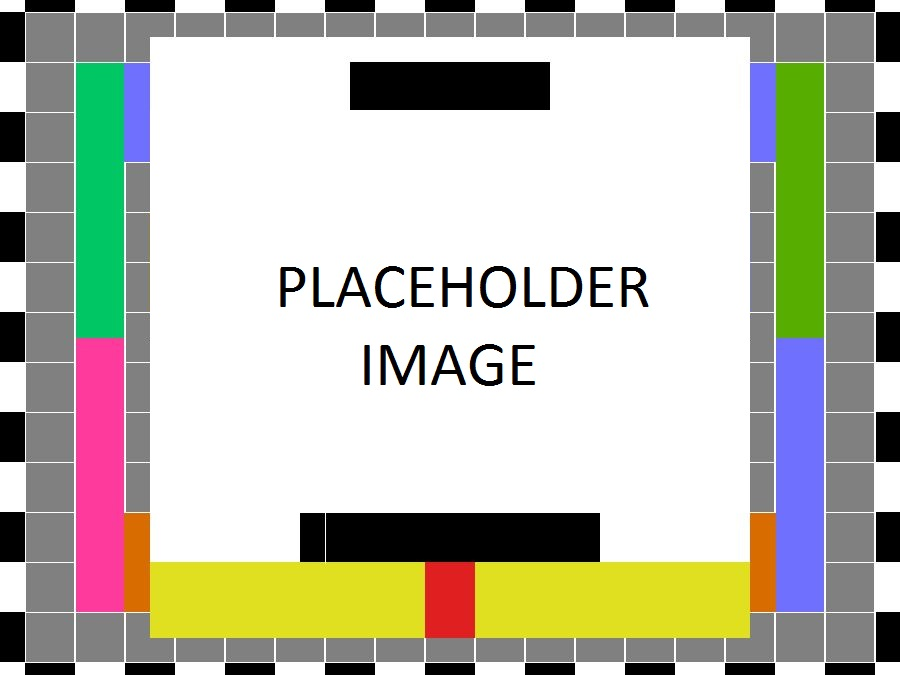
\includegraphics[width=0.60\textwidth]{images/test_image}
    \caption{X conceptual drawing} % Be sure to change the caption!
\end{figure}

\newpage
\section{Product Description}
This section provides a description of your product and defines it's primary features and functions. The purpose is to give the document reader/reviewer enough information about the product to allow them to easily follow the specification of requirements found in the remainder of the document. Your header for this section should introduce the section with a brief statement such as: "This section provides the reader with an overview of X. The primary operational aspects of the product, from the perspective of end users, maintainers and administrators, are defined here. The key features and functions found in the product, as well as critical user interactions and user interfaces are described in detail." Using words, and pictures or graphics where possible, specify the following:

\subsection{Features \& Functions}
What the product does and does not do. Specify in words what it looks like, referring to a conceptual diagram/graphic (Figure X).  Define the principle parts/components of the product. Specify the elements in the diagram/graphic that are part(s) of this product as well as any associated external elements (e.g., the Internet, an external web server, a GPS satellite, etc.)

\subsection{External Inputs \& Outputs}
Describe critical external data flows. What does your product require/expect to receive from end users or external systems (inputs), and what is expected to be created by your product for consumption by end users or external systems (outputs)? In other words, specify here all data/information to flow into and out of your systems. A table works best here, with rows for each critical data element, and columns for name, description and use.

\subsection{Product Interfaces}
Specify what all operational (visible) interfaces look like to your end-user, administrator, maintainer, etc. Show sample/mocked-up screen shots, graphics of buttons, panels, etc. Refer to the critical external inputs and outputs described in the paragraph above.

\newpage
\section{Customer Requirements}
% Size and Weight
% Sustainable Battery Life
% Easy of Use
% Wireless Connectivity
% Customization

The Roam\_Bot will be fully utilized by customers who have their own path finding system or some understanding of the movement of the rover. The rover will be able to navigate through set paths as well as the option to manually control where the rover will go.
%Include a header paragraph specific to your product here. Customer requirements are those required features and functions specified for and by the intended audience for this product. This section establishes, clearly and concisely, the "look and feel" of the product, what each potential end-user should expect the product do and/or not do. Each requirement specified in this section is associated with a specific customer need that will be satisfied. In general Customer Requirements are the directly observable features and functions of the product that will be encountered by its users. Requirements specified in this section are created with, and must not be changed without, specific agreement of the intended customer/user/sponsor.

\subsection{Reliable Movement}
\subsubsection{Description}
The Roam\_Bot will have motors controlling the 4 wheels of the rover. The motors are powered by a LiPo (Lithium Polymer 22.2V) battery. The power of the motors are controlled by a raspberry pi which takes in user input from our UI. 
% A detailed description of the feature/function that satisfies the requirement. For example: \textit{The GUI background will be slate blue. This specific color is required in order to ensure that the GUI matches other similar software products offered by the customer. Slate blue is specified as \#007FFF, using six-digit hexadecimal color specification.} It is acceptable and advisable to include drawings/graphics in the description if it aids understanding of the requirement.
\subsubsection{Source}
 CSE Senior Design project specifications
\subsubsection{Constraints}
The rover is limited by it's size and the overall cost of making a similar product. The wheels of the rover does not have a function to go up or down stairs easily.
%A detailed description of realistic constraints relevant to this requirement. Economic, environmental, social, political, ethical, health \& safety, manufacturability, and sustainability should be discussed as appropriate.
\subsubsection{Standards}
The speed of the motors will be limited so that it won't be a hazard when used incautiously. There will be a kill switch to turn off the rover in any situation and its function must not depend on any power source or wiring connection. The rover will meet strict cleanliness requirements to avoid contaminating samples with materials from Earth. The rover will not include any flammable, environmentally damaging, or otherwise hazardous liquids or gases.
%A detailed description of any specific standards that apply to this requirement (e.g. \textit{NSTM standard xx.xxx.x. color specifications \cite{Rubin2012}}. Standards exist for practically everything (ATC standard fuses, IEEE 802.15.4 embedded wireless, TLS 1.3 encryption, etc.), so be sure that you research and document which ones will be followed in meeting this requirement.
\subsubsection{Priority}
Priority Level: Critical (1)
%Use the following priorities:
%\begin{itemize}
 %\item Critical (must have or product is a failure)
 %\item High (very important to customer acceptance, desirability)
 %\item Moderate (should have for proper product functionality);
 %\item Low (nice to have, will include if time/resource permits)
 %\item Future (not feasible in this version of the product, but should be considered for a future release).
%\end{itemize}

\subsection{Path finding system}
\subsubsection{Description}
The path finding algorithm finds the shortest distance to the target spot while also noting the terrain around it to avoid while moving. The path finding algorithm will take in input from LIDAR and close range sensors. With the information, it will control the wheels to go in that direction.
\subsubsection{Source}
 CSE Senior Design project specifications
\subsubsection{Constraints}
Having the rover to constantly detect the path will slow processing power.
\subsubsection{Standards}
The factors that affect performance of the path finding system include the problem size, path length, number of obstacles, data structures, and heuristics.
\subsubsection{Priority}
Priority Level: High (2) (very important to customer acceptance, desirability)


\subsection{Attachments}
\subsubsection{Description}
The rover will have attachable components to help it navigate and perform different task. These attachments ranges from a water pump, a push arm, and any future attachments.
\subsubsection{Source}
 CSE Senior Design project specifications
\subsubsection{Constraints}
The amount of space the rover has and the carry weight of the rover limits what can be put on the rover.
\subsubsection{Standards}
The rover will not include any flammable, environmentally damaging, or otherwise hazardous liquids or gases.
\subsubsection{Priority}
Priority Level: Moderate (3) (should have for proper product functionality);

\newpage
\section{Packaging Requirements}
Include a header paragraph here. Packaging requirements are those requirements that identify how the delivered product will be packaged for delivery to the end-user; or how it will "look" when finished and delivered. For example, you might specify that the software required for operation will be pre-loaded on the hard drive, delivered on CD/DVD, or available via download. Software might be customer installable, or not, etc. Hardware components could be all in a single package, provided as a "bag of parts" to be assembled/installed by the user, painted a certain color, logos affixed, etc. Care should be taken not to duplicate requirements found in other sections of this document.

\subsection{Requirement Name}
\subsubsection{Description}
Detailed requirement description...
\subsubsection{Source}
Source
\subsubsection{Constraints}
Detailed description of applicable constraints...
\subsubsection{Standards}
List of applicable standards
\subsubsection{Priority}
Priority
\newpage
\section{Performance Requirements}
% Speed
% Navigation Accuracy
% Obstacle Avoidance
% Load Capacity
% Terrain Adaptability

The Roam\_Bot, is a rover that uses advanced pathfinding algorithms including Dijkstra's, Depth-First Search (DFS), Breadth-First Search, and A*. The purpose is to navigate environments autonomously. Designed for efficient navigation, the rover must meet specific operational metrics: completing path calculations within critical response times, achieving optimal setup and startup durations, maximizing battery life for extended deployment, and ensuring smooth and precise movement adjustments.

\subsection{Pathfinding}
\subsubsection{Description}
%The battery must be durable and able to survive extended periods of up to one hour without any further charging. It must also be able to withstand weathering conditions including erosion, damp environments, and temperature changes over times of inactivity.
This section details the performance requirements for the pathfinding algorithms.
\subsubsection{Source}
Team TLC
\subsubsection{Constraints}
The rover should follow these constraints:
\begin{itemize}
  \item The rover should be able to initialize calculating paths within 1000ms. 
  \item The rover should be able to recalculate paths after reaching its LIDAR range within 500-1200-ms.
  \item The rover should be limited to a max speed of 1 meter per second (m/s)
  \item Total weight should not exceed what the motors can handle effectively.
\end{itemize}
\subsubsection{Standards}
The rover should ensure it complies with:
\begin{itemize}
  \item Robot Operating System (ROS) Communication Protocols \cite{ROSCOM}
  \item Robot Operating System (ROS) Navigation Stack \cite{ROSCOM}
\end{itemize}
\subsubsection{Priority}
Priority Level: Critical (1)

\subsection{Battery Life}
\subsubsection{Description}
The battery system of the autonomous rover must deliver reliable power to support uninterrupted operation across varied terrains and usage scenarios.
\subsubsection{Source}
Team TLC
\subsubsection{Constraints}
\begin{itemize}
  \item Battery should last at least 4 hours of continuous operation.
  \item Recharge time should be under 4 hours to enable quick redeployment.
  \item The battery must perform reliably between -10°C and 50°C, with heat management solutions to prevent performance degradation in extreme conditions.
\end{itemize}
\subsubsection{Standards}
\begin{itemize}
    \item IEC 60086 \cite{IECBATT}
\end{itemize}
\subsubsection{Priority}
Priority Level: Future (5)

\newpage
\section{Safety Requirements}
% Emergency Stop (Yes)
% LiPo Battery Safety (Yes)
% Overcurrent Protection (Maybe???)
% Power Indicator (Maybe???)
% Fall Protection (Maybe???)
% IEC 60529 (Water and Particle Protection) (Maybe???)

% Include a header paragraph specific to your product here. Safety requirements might address items specific to your product such as: no exposure to toxic chemicals; lack of sharp edges that could harm a user; no breakable glass in the enclosure; no direct eye exposure to infrared/laser beams; packaging/grounding of electrical connections to avoid shock; etc.

The Roam\_Bot is designed to avoid any hazardous materials and breakable components including glass. All electrical components will be properly protected and grounded to prevent any unwanted current discharge. If the robot's action becomes undesirable, safety protocols are implemented for an emergency stop to prevent further robot or human injury.



\subsection{Laboratory Equipment Lockout/Tagout (LOTO) Procedures}
\subsubsection{Description}
% Description of the Requirement
Any fabrication equipment provided used in the development of the project shall be used in accordance with OSHA standard LOTO procedures. Locks and tags are installed on all equipment items that present use hazards, and ONLY the course instructor or designated teaching assistants may remove a lock. All locks will be immediately replaced once the equipment is no longer in use.

\subsubsection{Source}
% The source of the requirement (e.g. customer, sponsor, specified team member (by name), federal regulation, local laws, CSE Senior Design project specifications, etc.)
CSE Senior Design Laboratory Policy

\subsubsection{Constraints}
% A detailed description of realistic constraints relevant to this requirement. Economic, environmental, social, political, ethical, health \& safety, manufacturability, and sustainability should be discussed as appropriate.
Equipment usage, due to lock removal policies, will be limited to the availability of the course instructor and designed teaching assistants.

\subsubsection{Standards}
% A detailed description of any specific standards that apply to this requirement (e.g. \textit{NSTM standard xx.xxx.x. color specifications \cite{Rubin2012}}. Standards exist for practically everything (ATC standard fuses, IEEE 802.15.4 embedded wireless, TLS 1.3 encryption, etc.), so be sure that you research and document which ones will be followed in meeting this requirement.
Occupational Safety and Health Standards 1910.147 - Control of Hazardous Energy (Lockout/Tagout).

\subsubsection{Priority}
% Critical (1)
% High (2)
% Moderate (3)
% Low (4)
% Future (5)
Priority Level: Critical (1)



\subsection{National Electric Code (NEC) Wiring Compliance}
\subsubsection{Description}
Any electrical wiring must be completed in compliance with all requirements specified in the National Electric Code. This includes wire runs, insulation, grounding, enclosures, over-current protection, and all other specifications.

\subsubsection{Source}
CSE Senior Design Laboratory Policy

\subsubsection{Constraints}
High voltage power sources, as defined in NFPA 70, will be avoided as much as possible in order to minimize potential hazards.

\subsubsection{Standards}
NFPA 70

\subsubsection{Priority}
Priority Level: Critical (1)
\newpage



\subsection{Emergency Stop}
\subsubsection{Description}
This easily accessible switch is designed to stop all power, turning the robot off immediately. This feature will disconnect the battery despite the current state of the robot.

\subsubsection{Source}
Team TLC

\subsubsection{Constraints}
Accessibility: The button is made easily accessible to all users, ensuring quick activation in an emergency.\\
Health and Safety: The stop is designed to protect all users by providing a nearly instant stop to all robot activity, reducing the risk of human injury.

\subsubsection{Standards}
- ISO 13850 (Safety of Machinery)\\
- ANSI/RIA R15.06 (Safety of Robot Systems)

\subsubsection{Priority}
Priority Level: Critical (1)



\subsection{LiPo Battery Safety}
\subsubsection{Description}
The battery is handled safely throughout its lifecycle, including its use, physical handling, and charging.

\subsubsection{Source}
Team TLC

\subsubsection{Constraints}
Environmental: LiPo batteries must be used and disposed of following industry standards to reduce their environmental impact and support the sustainability of recycling.\\
Health and Safety: Safety measures are followed when charging and using the LiPo batteries to prevent the release of dangerous currents.

\subsubsection{Standards}
- IEC 62133 (Safety for Lithium Batteries)\\
- UN 38.3 (Transport Safety for Lithium Batteries)

\subsubsection{Priority}
Priority Level: Critical (1)

\newpage
\section{Maintenance \& Support Requirements}
Include a header paragraph specific to your product here. Maintenance and support requirements address items specific to the ongoing maintenance and support of your product after delivery. Think of these requirements as if you were the ones who would be responsible for caring for customers/end user after the product is delivered in its final form and in use "in the field". What would you require to do this job? Specify items such as: where, how and who must be able to maintain the product to correct errors, hardware failures, etc.; required support/troubleshooting manuals/guides; availability/documentation of source code; related technical documentation that must be available for maintainers; specific/unique tools required for maintenance; specific software/environment required for maintenance; etc.

\subsection{Requirement Name}
\subsubsection{Description}
Detailed requirement description...
\subsubsection{Source}
Source
\subsubsection{Constraints}
Detailed description of applicable constraints...
\subsubsection{Standards}
List of applicable standards
\subsubsection{Priority}
Priority
\newpage
\section{Other Requirements}
Include a header paragraph specific to your product here. In this section specify anything else that is required for the product to be deemed complete. Include requirements related to customer setup and configuration if not specified in a previous requirement. Add any known requirements related to product architecture/design, such as modularity, extensibility (for future enhancements), or adaptation for a specific programming language. Consider requirements such as portability of your source code to various platforms (Windows, Linux, Unix Mac OS, etc.).

\subsection{Requirement Name}
\subsubsection{Description}
Detailed requirement description...
\subsubsection{Source}
Source
\subsubsection{Constraints}
Detailed description of applicable constraints...
\subsubsection{Standards}
List of applicable standards
\subsubsection{Priority}
Priority
\newpage
\section{Future Items}
% Advanced AI (Maybe???)
% Autonomous Charging (Maybe???)
% Cloud Connectivity (Maybe???)
% Extended Sensing Capabilities (Maybe???)

% In this last section, you will reiterate all requirements that are listed as priority 5. This is repetitive, but necessary as a concise statement of features/functions that were considered/discussed and documented herein, but will NOT be addressed in the prototype version of the product due to constraints of budget, time, skills, technology, feasibility analysis, etc. Use the following format for this section.



%%%%%%%%%% Reiterated Requirements From: Performance
\subsection{Battery Life}
\subsubsection{Description}
The battery system of the autonomous rover must deliver reliable power to support uninterrupted operation across varied terrains and usage scenarios.
\subsubsection{Source}
Team TLC
\subsubsection{Constraints}
\begin{itemize}
  \item Battery should last at least 4 hours of continuous operation.
  \item Recharge time should be under 4 hours to enable quick redeployment.
  \item The battery must perform reliably between -10°C and 50°C, with heat management solutions to prevent performance degradation in extreme conditions.
\end{itemize}
\subsubsection{Standards}
\begin{itemize}
    \item IEC 60086 \cite{IECBATT}
\end{itemize}
\subsubsection{Priority}
Priority Level: Future (5)




%%%%%%%%%% Reiterated Requirements From: Maintenance & Support
\subsection{Diagnostics Tools}
\subsubsection{Description}
These tools will provide an easy way to identify major problems in hardware or software that can prevent the robot from functioning safely.
\subsubsection{Source}
Team TLC
\subsubsection{Constraints}
Environmental: The diagnostics are used to ensure the health of the robot, preventing unnecessary waste from the early replacement of components.\\
Economic: The cost of diagnostics tools should remain within the robot budget.\\
Sustainability: The diagnostics should minimize the need for replacements, allowing the robot to function for longer periods of time.
\subsubsection{Standards}
- IEC 61010 (Safety Requirements for Electrical Measurement)\\
- IEEE 802.3 (Wired Communication Protocols)\\
- ISO 9001 (Reliable Quality Measurements)
\subsubsection{Priority}
Priority Level: Future (5)

\newpage

%%% References
\bibliographystyle{reference/IEEEtran_custom}
\bibliography{reference/refs}{}


\end{document}
